% !TeX root = ../main.tex

\chapter{Source-Heterogeneity Examination}

Figure 7.1 shows that the behavior between different newspapers is quite diverse. Liberty Times tends to have dramatic response to the GPR event, and sometimes reach zero related articles. However, China Times and United Daily have a consistent interest in GPR news while creating smaller spikes.
Figure 7.2 shows the raw article counts for each newspaper that contributes to the GPR index. The large discrepancy indicates that each newspaper has a different content creation policy. The dramatic drop of Liberty Times news count may indicates the media's policy shift or the policy for bot crawling had changed. The consistently higher count of China Times articles actually comes from its policy to farm content. The missing data after 2024, is its policy change to block CC-NEWS crawler which is common after ChatGPT released. The different media properties suggest that conducting \citet{caldara}'s original method to treat all articles equal from different newspapers need more research in Taiwan's case.
Another evidence is the corelation score is much lower than  \citet{caldara}'s finding in US case.

\begin{figure}[htbp]
  \centering
  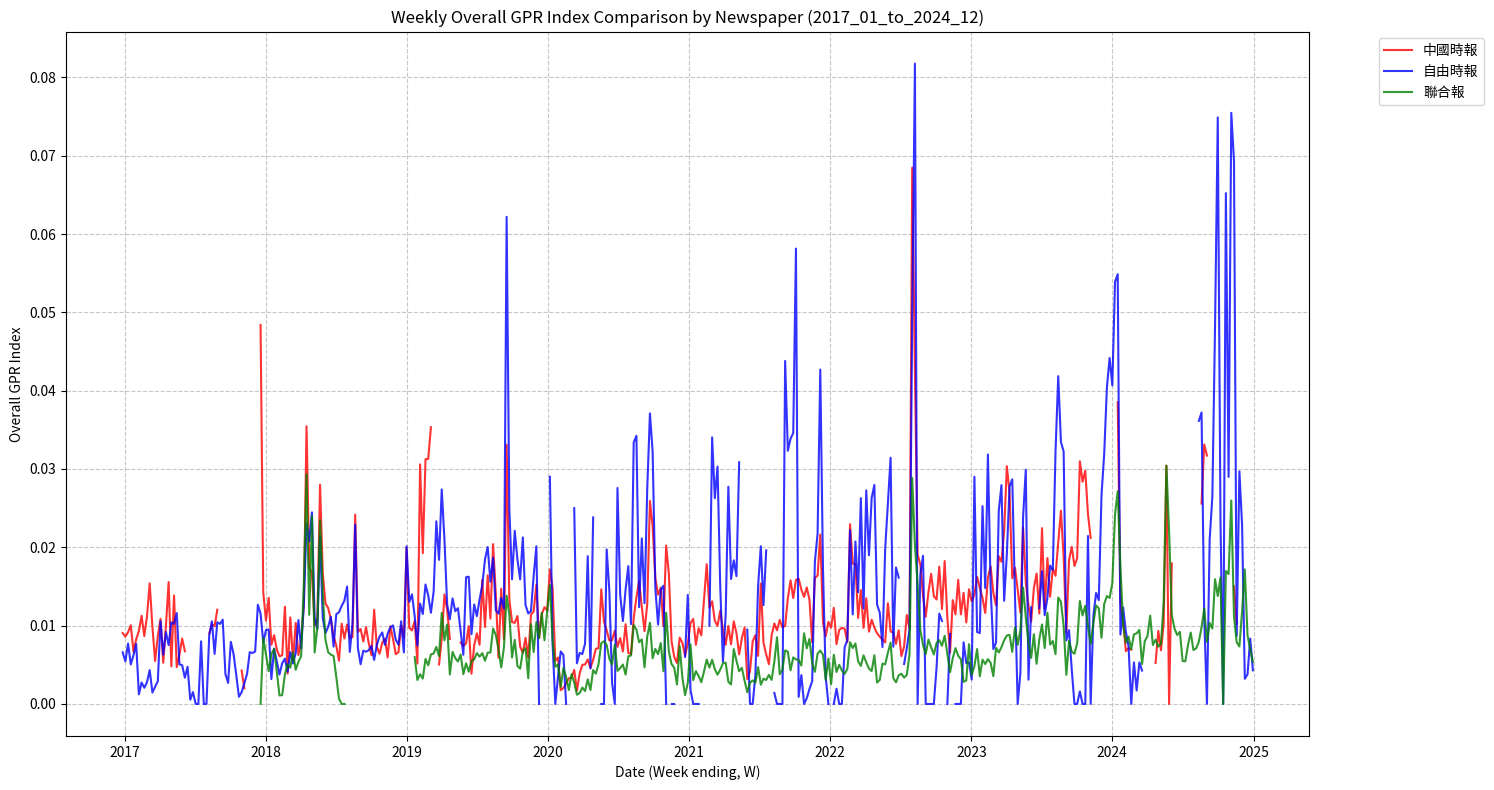
\includegraphics[width=\linewidth]{gpr_index_comparison_all_newspapers_2017_01_to_2024_12.png}
  \caption{GPR Index for each newspaper}
  \label{fig:my_example}
\end{figure}

\begin{figure}[htbp]
  \centering
  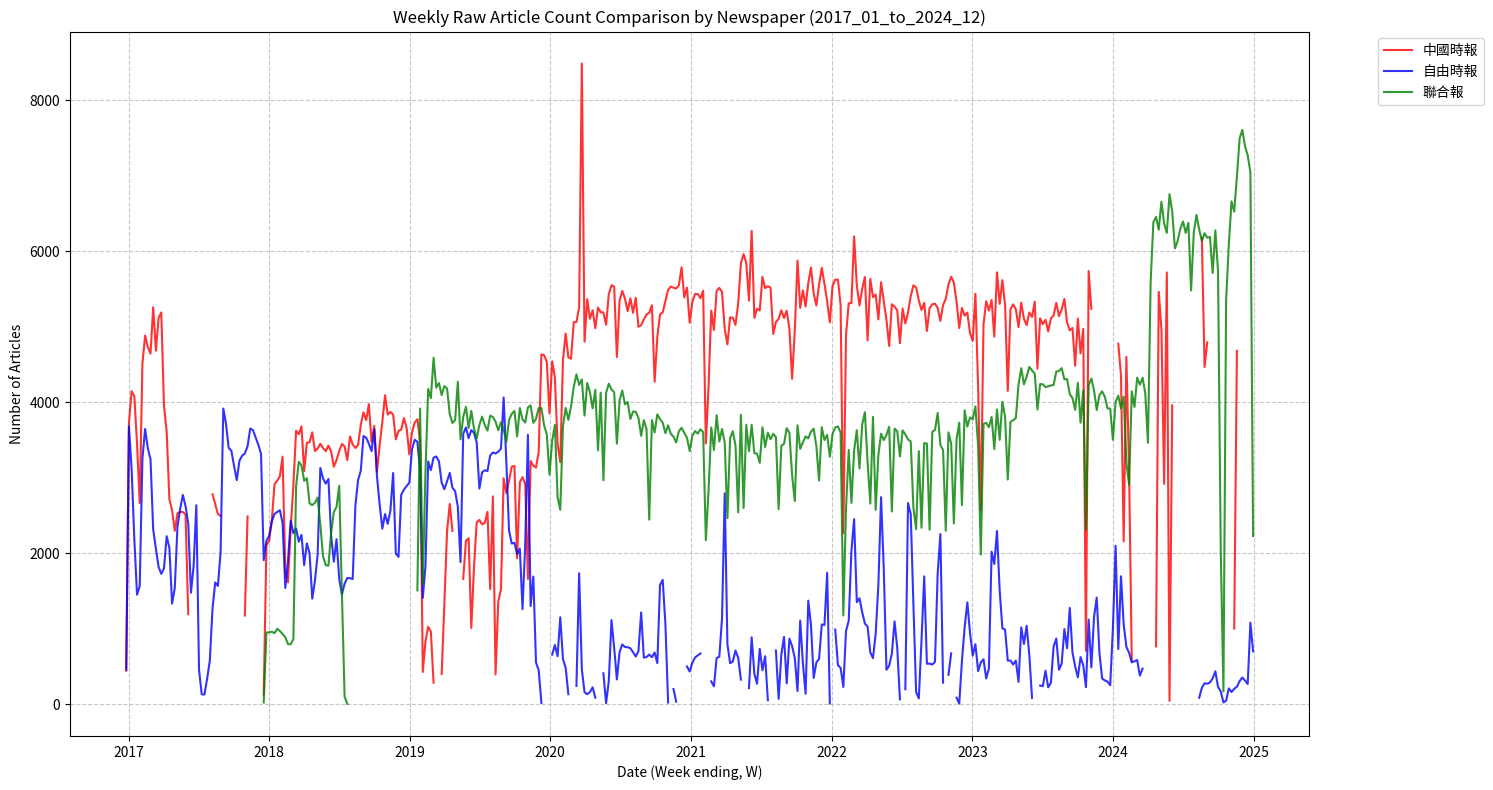
\includegraphics[width=\linewidth]{article_count_comparison_all_newspapers_2017_01_to_2024_12.png}
  \caption{Articles count for each newspaper}
  \label{fig:my_example}
\end{figure}